%%%%%%%%%%%%%%%%%%%%%%%%%%%%%%%%%%%%%%%%%%%%%%%%%%%%%%%%%%%%%%%%%%%%%%
%\section{Prototyping}
%%%% Matt
%
%%%%%%%%%%%%%%%%%%%%%%%%%%%%%%%%%%%%%%%%%%%%%%%%%%%%%%%%%%%%%%%%%%%%%%
%\section{Installation and Commissioning}
%%%% Patrick

%%%%%%%%%%%%%%%%%%%%%%%%%%%%%%%%%%%%%%%%%%%%%%%%%%%%%%%%%%%%%%%%%%%%%
\section{Costing}
%%% Matt

%%%%%%%%%%%%%%%%%%%%%%%%%%%%%%%%%%%%%%%%%%%%%%%%%%%%%%%%%%%%%%%%%%%%%
\subsection{M\&S}

Table \ref{tab:baseMScost} shows the cost estimate for the RCE/ATCA hardware.  The estimates for the COB and DTM are based on actual units that have been produced for the LSST experiment.  Costs for the DPM and RTM are estimates based on past production of similar parts and quotes for the new components (FPGA, memory and SSDs).  The crate cost,  with power supplies and shelf manager, is based on past purchases.  

\begin{table}[htp]
\begin{center}
\begin{tabular}{|c|c|c|c|c|}
\hline
 Name  & Quantity & Turnkey Quote(\$/unit)      & Parts(\$/unit)            &     Cost/SP 10kT (\$) \\
  \hline
COB		&  150 	&	5,035		&	1,625		&	999,000\\
\hline
DTM		&  150 	&	595		&	148		&	111,413\\
\hline
DPM		&   600	&	892		&	1969		&1,715,832	\\
\hline
RTM		&   150	&	1,000		&	0		&150,000	\\
\hline
Crate		&   11	&	8,500		&	0	&	93,500	\\
\hline
\hline
{\bf Total } &	\multicolumn{3}{r|}{} & {\bf 3,069,745}   \\
\hline
{\bf Cost/COB }& 	\multicolumn{3}{r|}{} &  {\bf  20,465 }  \\
\hline
\end{tabular}
\end{center}
\caption{ Costing estimates of the COBs and related hardware for the base RCE/ATCA system (1 RCE/DPM) presented here. }
\label{tab:baseMScost}
\end{table}%

We also include a table of hardware cost estimates for the dual-RCE/DPM system described in Section \ref{sec:upgrades}.  As shown, the estimated cost of the hardware is reduced by $\sim$\$1M with very little change in firmware or software needed.  


\begin{table}[htp]
\begin{center}
\begin{tabular}{|c|c|c|c|c|}
\hline
 Name  & Quantity & Turnkey Quote(\$/unit)      & Parts(\$/unit)            &     Cost/SP 10kT (\$) \\
  \hline
COB		&  75 	&	5,035		&	1,625		&	499,500\\
\hline
DTM		&  75 	&	595		&	148		&	55,706\\
\hline
DPM		&   300	&	892		&	3,539		&1,329,216	\\
\hline
RTM		&   75	&	1,000		&	0		&75,000	\\
\hline
Crate		&   6	&	8,500		&	0	&	51,000	\\
\hline
\hline
{\bf Total } &	\multicolumn{3}{r|}{} & {\bf 2,010,422}   \\
\hline
{\bf Cost/COB }& 	\multicolumn{3}{r|}{} &  {\bf  26,806 }  \\
\hline
\end{tabular}
\end{center}
\caption{ Costing estimates of the COBs and related hardware for the high-density RCE/ATCA system (2 RCE/DPM) presented as an upgrade to the base solution. }
\label{tab:HDMScost}
\end{table}%


%%%%%%%%%%%%%%%%%%%%%%%%%%%%%%%%%%%%%%%%%%%%%%%%%%%%%%%%%%%%%%%%%%%%%
\subsection{Labor}

Table \ref{tab:basecostLabor} shows a breakdown of estimate engineer or technician labor needed for this project.  The timescale is from now (roughly start of FY19) until 
2024 (when the first detect is scheduled to be complete).   We haven't included non-expert (i.e. physicists) labor here but expect we should have 2-3 FTE of graduate student, post-doc or staff level who are "experts" on the system at all times during the integration, installation and commissioning phases.  

\begin{table}[htp]
\begin{center}
\begin{tabular}{|c|c|l|}
\hline
 Description of Task  &Estimated    &  Notes\\
& FTE-months &  \\
 \hline
\hline
\multicolumn{3}{|l|}{\bf Hardware}   \\
\hline
 Ultra-scale DPM testing \& validation &  2      & To begin soon at Oxford soon\\
  \hline 
  Ultra-scale DPM second spin  &  3      & Likely needed, includes testing \& validation\\
  \hline 
    Rear-Transition Module Design  &  0.5    &  After WIB and timing interfaces  \\
    &&have been fixed; based on past designs\\
\hline
\hline
\multicolumn{3}{|l|} {\bf RCE Firmware}   \\
\hline
Ultrascale upgrades to core RCE firmware     & 2 & Incorporate improvements \\
\hline
WIB-RCE data interface   & 0.25&  Higher destiny and format changes (if any) \\
\hline
Compression   & 3 & Add slimmer  engine \\
\hline
Trigger Primitive Finding   & 3 &Including formatting and DMA \\
\hline
Buffering   &  3  &  Improved buffer management \\
\hline
\hline
\multicolumn{3}{|l|} {\bf RCE Software}   \\
\hline
Switch to Rogue	&	2	&	Currently using old C++-based software \\
\hline
Trigger Primitive Data Path	&	1	&Output from memory to backend via RSSI \\
\hline
Triggered Data Path	&	1	&		Output from memory to backend via RSSI \\
\hline
SN Data Path:  to SSD &	3	&	 Output from memory to SN SSD via PCIe bus \\
\hline
SN Data Path:  from SSD &	3	&	Output from SN SSD to backend via RSSI \\
\hline
\hline
\multicolumn{3}{|l|} {\bf Testing \& Integration}   \\
\hline
RCE Slice Testing	&	3	&	Full firmware and software chain \\
\hline
DAQ VST Support	&	6	&	Integration with other hard/soft components \\
\hline
Non-DAQ Test stands	&	6	&	Support for CE testing\\
\hline
\hline
{\bf Total FTE-months pre-install}&   41.75  & \\
\hline
\hline 
\multicolumn{3}{|l|}{\bf Installation \& Commissioning}   \\
\hline
Integration, Installation \& Commissioning  & 36  & Continually at some level 2019-2024\\
\hline
\hline
\end{tabular}
\end{center}
\caption{ Labor estimates for the base RCE/ATCA design.  All FTE are for engineers or technicians. }
\label{tab:basecostLabor}
\end{table}%




%%%%%%%%%%%%%%%%%%%%%%%%%%%%%%%%%%%%%%%%%%%%%%%%%%%%%%%%%%%%%%%%%%%%%
%\section{Schedule}
%%% Matt

%%%%%%%%%%%%%%%%%%%%%%%%%%%%%%%%%%%%%%%%%%%%%%%%%%%%%%%%%%%%%%%%%%%%%
\section{Extensions and Upgrades}
\label{sec:upgrades}
%%% Matt

There are some extensions to the base design described above that could be made, both in hardware and software.  These are described below. 

\subsection{Adding the artDAQ boardReader to the RCE}
\label{sec:board reader}
The artDAQ software suite is the most likely choice to be used for the backend DAQ.  artDAQ consists of three main part:  a boardReader which reads from the electronics (in this case, the RCEs), an eventBuilder which collects the fragments from the boardReaders and assembles them into events, and an Aggregator which takes the build events and writes them to disk.  In both the 35ton and protoDUNE prototypes, the each of these stages ran on different tiers of PCs.  However, it should be possible to include the boardReader stage on the RCEs themselves, eliminating a tier of PCs for the triggered data path. 

Implementing the boardReader on the RCEs will mainly involve working to build the needed artDAQ packages and their dependencies on the ARM/ArchLinux architecture.  Fermilab CD scientists had begun investigating the feasibility of this but shifted focus to the protoDUNE DAQ project.  This task will likely require a combination of artDAQ, Fermilab CD and  RCE experts and careful version control and management from both sides.  

\subsection{Including Trigger Decision Processing on RCE Cluster}
\label{sec:triggerOnRCE}
 As mentioned above,  each RCE has a significant CPU onboard. The base design (even with the boardReader process) should use very few of these computing resources; basically it is just directing traffic between streams.  The high-speed links connecting each RCE (10 or even 40 Gbps, depending on the choice of switch) could make the COB platform a good place to do a first level of the trigger decision processing.  Actions such as clustering of trigger primitives and, since  each COB deals with at least 1 APA's worth of data (or two, see below), APA-level decisions could be performed.  
 
 This project would take significant effort but likely doesn't require much RCE-expert level intervention to complete.  

\subsection{Dual-RCE DPM}
\label{sec:dualRCE}
We believe it's possible to put two of the Ultrascale-RCEs on a single DPM which would have considerable cost savings over the single-RCE DPM currently in production.  This is not unprecedented as the Gen-3 DPMs, used in 35-ton and protoDUNE, carry 2 RCEs/DPM.  

The concept art for this design is shown in Figure \ref{fig:dualRCE}.  While this design is almost duplicated from the single-RCE/DPM design, there is only room on the board for a single chip of DDR4 memory.  There are some risks associated with making the board more dense (heat load, power usage/COB) but they are low.  Going to a single chip of 8GB of memory reduces our buffer size, reducing the latency we can allow for triggers though by the time these would go into production 16GB chips may become available and cost-effective.  

\begin{figure}[tb]
\centering
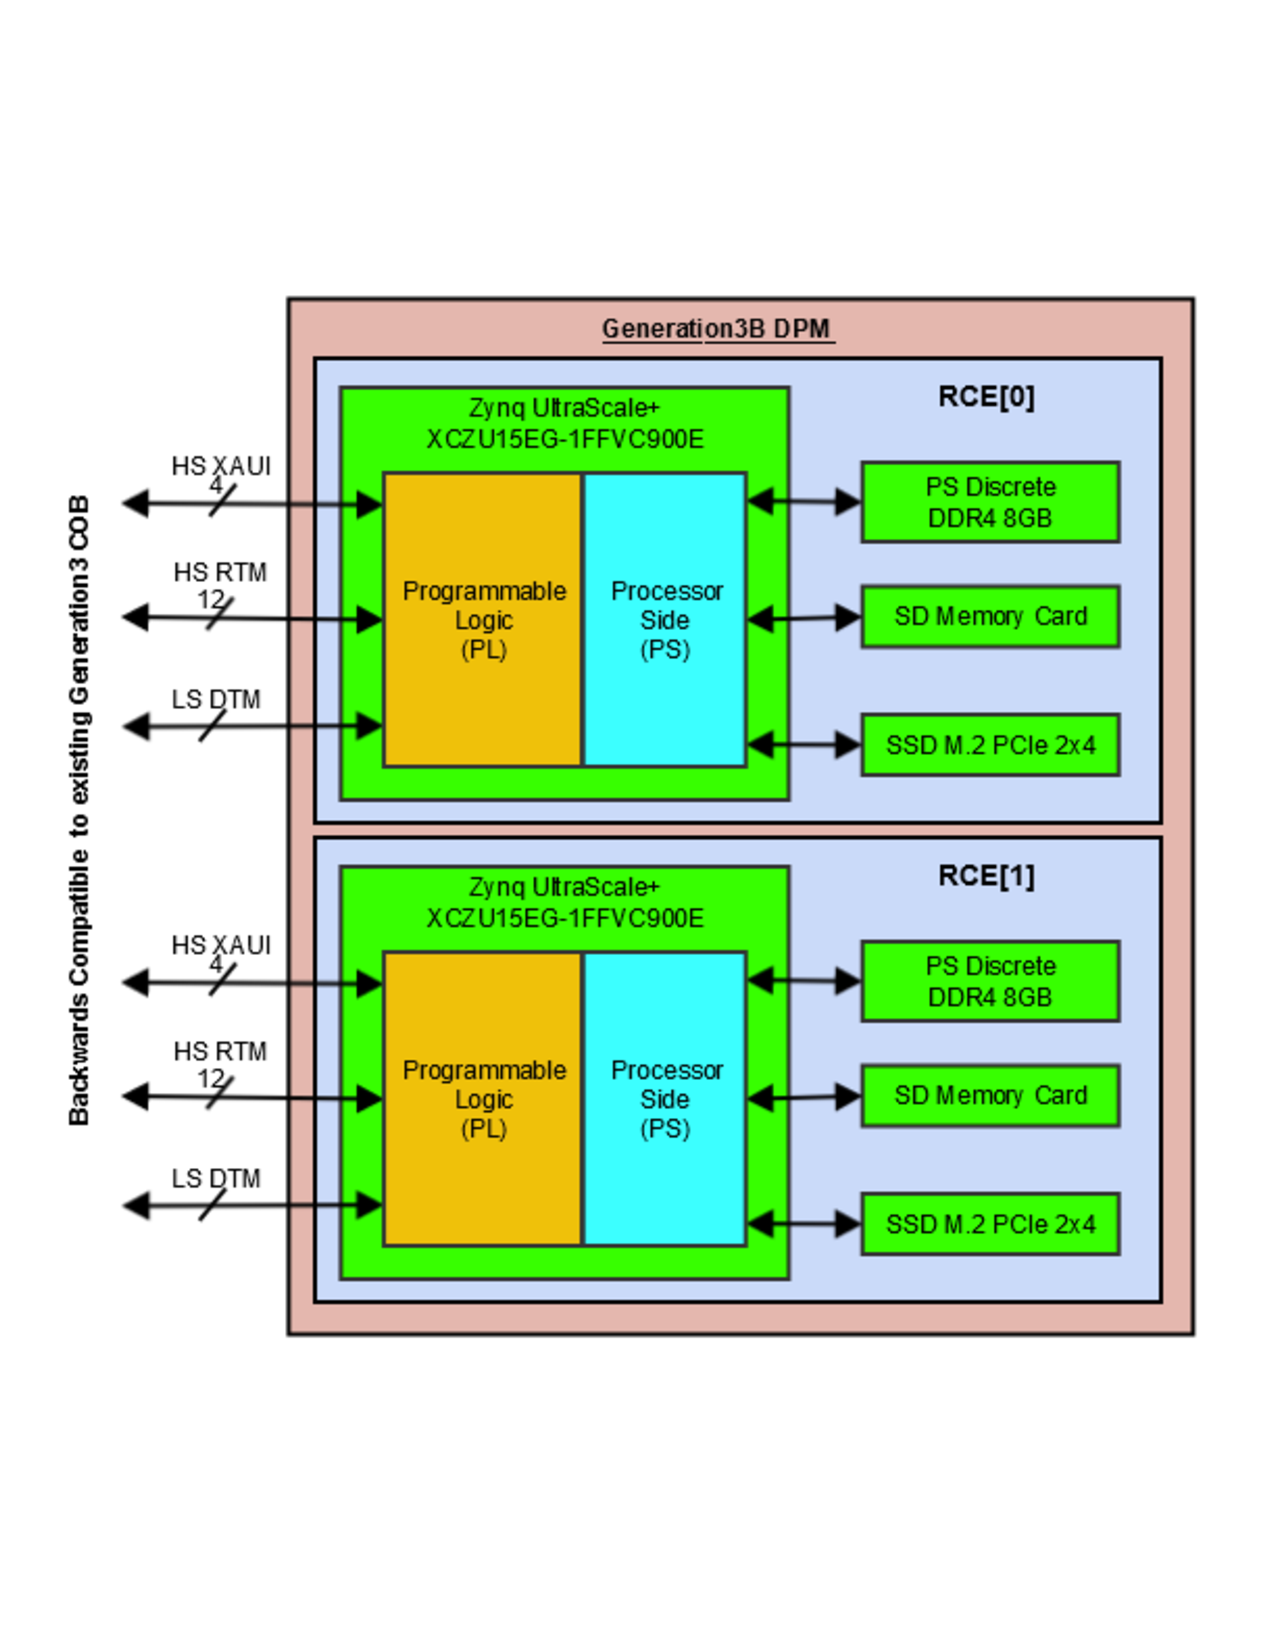
\includegraphics[width=0.5\textwidth]{images/dual-RCE-DPM.pdf}.
\caption{\label{fig:dualRCE}Block diagram and concept art of the dual-RCE DPM.}
\end{figure}

The cost breakdown of the dual-RCE design is shown in Table \ref{tab:HDMScost}.  The reduction in cost primarily comes from the halving of each item of equipment needed: the COBs, RMTs, and crates.  The dual-RCE design would also obviously take half the rack space necessary and somewhat reducing the total power need. 

%%%%%%%%%%%%%%%%%%%%%%%%%%%%%%%%%%%%%%%%%%%%%%%%%%%%%%%%%%%%%%%%%%%%%
\section{Summary}
%%% Mark

%%%%%%%%%%%%%%%%%%%%%%%%%%%%%%%%%%%%%%%%%%%%%%%%%%%%%%%%%%%%%%%%%%%%%

\bibliographystyle{alpha}
\bibliography{sample}

%%%%%%%%%%%%%%%%%%%%%%%%%%%%%%%%%%%%%%%%%%%%%%%%%%%%%%%%%%%%%%%%%%%%%

